\section{Resident Evil}

\begin{figure}[htbp]
\begin{center}
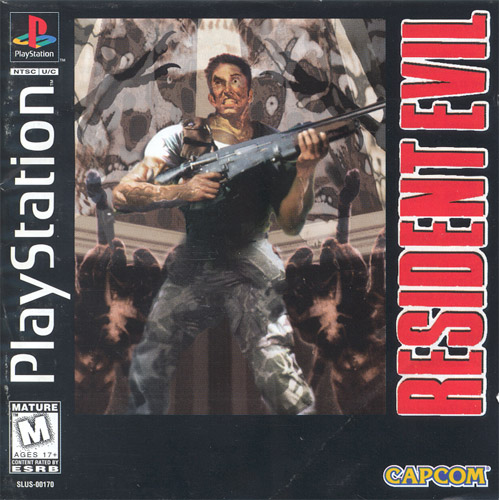
\includegraphics[width=.35\textwidth]{./imagenes/resident_evil1.jpg}
\caption{Resident Evil}
\label{Resident Evil}
\end{center}
\end{figure}
Una extraña ola de asesinatos empiezan a ocurrir en las montañas Arklay a las afueras de Racoon City.  Es entonces que la noche del 24 de julio de 1998 el departamento de policia de Racoon City envia al equipo Bravo del gurpo especial S.T.A.R.S. (Special Tactics And Rescue Service) a investigar. Al poco tiempo se pierde el contacto con el equipo Bravo y se envia al equipo Alpha a continuar la investigacion y encontrar al equipo Bravo. Al llegar son atacados por una especie de perros zombies y son obligados a refugiarse en una mansion cercana. Es Aqui Donde comienza la pesadilla de los S.T.A.R.S. por sobrevivir ya que la mansion es un centro secreto de desarrollo de armas biologicas, y los miembros de S.T.A.R.S. han sido engañados para probar una nueva arma denominada Virus-T la cual es capaz de reviir el tejido muerto a nivel celular. En Resident Evil\footnote{\url{http://www.residentevilcenter.net/residentevil.html}} entramos en la piel de los miembros del equipo Alpha de S.T.A.R.S. Chris Redfield o Jill Valentine los cuales se enfrentaran a monstruos creados con el virus-T tales como zombies y demas criaturas; con municion limitada y su sentido de supervivencia.

\subsubsection{¿Por qué es uno de mis juegos favoritos?}
\begin{itemize}
\item[Joseph Gallardo] Es un juego del genero Survival Horror el cual se caracteriza por su camara estatica, y la escasa municion la cual habra que utilizarla sabiamente, ya que habra ocasiones en las que sera mejor huir antes que pelear. La historia del juego es exelente, los puzzles son un verdadero reto y las desiciones que tomes durante el juego afectan al final de la historia. Es uno de mis videojuegos favoritos ya que lo considero como un verdadero reto para superar.
\end{itemize}